\chapter{Testing}

%Detailed descriptions of every test case are definitely not what is required here. What is important is to show that you adopted a sensible strategy that was, in principle, capable of testing the system adequately even if you did not have the time to test the system fully.

%Have you tested your system on �real users�? For example, if your system is supposed to solve a problem for a business, then it would be appropriate to present your approach to involve the users in the testing process and to record the results that you obtained. Depending on the level of detail, it is likely that you would put any detailed results in an appendix.

%The following sections indicate some areas you might include. Other sections may be more appropriate to your project.

This chapter discusses the testing strategy which has been implemented on the project. This includes unit, acceptance and user testing utilised throughout various parts of the application.

\section{Overall Approach to Testing}
To recape, an agile approach was adopted throughout the project. From the process, test-driven-development was used throughout the application for almost all aspects of testing.

\subsection{Test-driven-development}
Test-driven-development(TDD) was adopted throughout all aspects of the application. All implementation code as an test which covers the purpose of the implementation. Figure \ref{fig:tdd} shows the TDD cycle.

\begin{figure}
  \includegraphics[scale=0.5]{images/tdd}
  \centering
  \caption{The cycle of TDD during the development stages of the application}
  \label{fig:tdd}
\end{figure}

A sensible test was created and, following the cycle, this would fail when first tested. The following steps would be to ensure that the tests pass by adding the associated code needed to make sure that it passes - afterwards refactoring occurs to ensure that design is kept simple and as clean as possible for the current implementation.

This approach could have been modified so that a group of tests were created for a feature and then implement a set of functions. This testing strategy was rejected and a pure one test for one bit of functionality was used. This was mainly to ensure that the design was not being over complicated.

Reflecting on the testing strategy and the design, it really did help to think of the design through a test-driven-development way. It ensured that the domain was fully understood before creating a test. This left the codebase tested fully - through a variety of aspects.
\section{Automated Testing}
One thing to note is that Flask's testing documentation is very sparse and is of low quality.

During the first few iterations of tests pytest was originally being used to create test classes, making all the classes extent $unittest.TestCase$.

Flask tests were refactored mid-way through the series of sprints to use Flask-testing[Cite]. This offers better testing support for Flask application, allowing the creation of dummy application and providing the functionality to run a quick server for testing.

\section{Mocking Tests}
Mocking during tests is changing the output of a function to return a specific value which is known about [CITE]. It was established that certain tests would need to be mocked, because some data would change from test to test. It was identified that \textit{all} interactions with Google API's, any interactions with Tesseract and the Session would need to be mocked.

It is best practice when developing application that the developers should not hit a production URL during development and testing. As the Google API does not support specific environment API's, then all URLs would be to a production URL. The issue this raises when testing is ensuring that the tests are isolated and pass every time. For example, if the test queried the API one day it will return a specific result, but when queried another day it may return another result; this requires  mocks to be used. The mock would return a specific value every time, ensuring tests can be reliable.

The principle is the same for testing Tesseract in the web application. If more training was conducted then the results from the test on the image would change, therefore ensuring that the tests have consistency data was mocked from specific functions - to check they returned the correct output.

During the first few sprints, whilst understanding how mocks work with Python, there was a lot of duplication with the mocking services. The library mock [CITE] uses annotations above test functions to signal a mock value.

\begin{lstlisting}[language=python, caption={An example of using mocks, following the annotation pattern}, label={lst:mock1}, breaklines, columns=fullflexible, keywordstyle=\color{blue}]
  @mock.object(GoogleOauthService, 'authorise')
  @mock.object(GoogleCalendarService, 'execute_request')
  def test_return_correct_response(self, authorise, calendar_response):
    authorise.return_value = some_json
    calendar_response.return_value = some_more_json
\end{lstlisting}

Mocking example \ref{lst:mock1} shows the syntax which was initially used by the tests. This would result in many of the tests becomming unreadable and easy to follow exactly what the point was. Additionally the do not repeat yourself (DRY) principle was violated, by duplicating much of the codebase.

Looking the mock API documentation, patching object calls was discovered. Implementing this solution reduced the amount of code for mocking specific functions. The annotations were removed from the top of function tests. Initally it was not entirely clear how to implement these patch functions. Eventually the patch was included in the $setUp$ and $tearDown$ functions, as shown in figure \ref{lst:mock2}. The code for mocking is a lot more succinct.

\begin{lstlisting}[language=python, label={lst:mock2}, breaklines, columns=fullflexible, keywordstyle=\color{blue}, label={Mocks using the patch and start. It stops in the dear downs}]
    def setUp(self):
      # some code
      authorise_patch = mock.patch()
      authorise_mock = authorise_patch.start()
      authorise_mock.return_value = some_json


    def tearDown(self):
      mock.patch.stopAll()
\end{lstlisting}

Often when testing the code there needed to be ways in which the output varied depending on when it was called. In Python mock library they had the functionalty for that, and it was called side effects.

\begin{lstlisting}[language=python, label={lst:mock3}, breaklines, columns=fullflexible, keywordstyle=\color{blue}]
    def setUp(self):
      # some code
      self.google_patch = mock.patch.object(GoogleCalendarService, "execute_request")
          self.google_mock = self.google_patch.start()
          self.google_mock.side_effect = [self.google_response, self.new_event, self.google_response, self.updated_response]

    def teatDown(self):
      mock.patch.stopAll()
\end{lstlisting}

Figure \ref{lst:mock3} shows the use of the ``side effect''. It is essentially, a way to define a series of output. From the above exame, it outputs google response first, then when $execute_request$ is called for a second time $new_event$ response is fired and so on. This was implemented due to the way the code was implemented in the controller, where multiple calls to the same function were executed, but different results were needed from the calendar.

Overall, mocking produced a substantial amount of testing. It was not considered when designing the system that mocking would be needed, it was only when testing happened that it was realised it was needed. The tests were refactored to incorporate the mocking facilities.

\subsection{Unit Testing}
A Unit test is used for models where functions can be tested in isolation to ensure that they perform the correct operations. In the application unit tests were created for every model.

Sometimes there was a cross over between database transactions and testing specific functions. In these cases, using the actual database would not be used for testing against. This is not considered the best design [CITE], so a test database was initialised.

The config was overwritten to include $app.config['testing'] = True$ and $app.config['SQLALCHEMY_DATABASE_URI'] = 'sqlite:///test.sqlite'$. This ensured that a test database was used, which was cleared and created for every test - this ensured that the database did not influence other tests.

Very much like the function names of the classes, the test cases were as descriptive as possible. This formed part of the documentation of the application.

\begin{figure}[h]
  \centering
  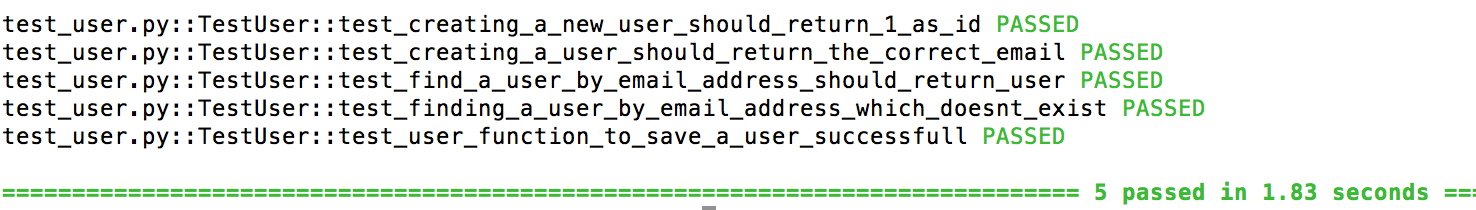
\includegraphics{images/unit_test_user}
  \caption{Example Unit test for the user class. Each of the tests pass}
  \label{fig:unit_user}
\end{figure}

Figure \ref{fig:unit_user} shows an example of the unit tests for the user class. The functions were decomposed and tests were associated for each function. In cases both edge-cases and normal expected results were selected.

Refer to appendix x for full unit test cases.

\subsection{Integration Testing}
Due to the application having external routes, then testing them to ensure the correct response codes was important. These were the first tests written for the routing sections, and implemented from the design considerations in X.

The tests consisted of checking that the response code was correct, any that redirects were correctly redirected to test the flow of the application.

Where there was integrations with the database in the routes, then tests were conducted to ensure the routes performed the correct persistance. For example, when posting to the meta-data URL, then checks were created to ensure that the module code was being persisted correctly.

\subsection{Handling sessions}
One of the tricker aspects of testing was the handling of sessions. In parts of the application sessions are used to handle specific states of the system, i.e when a user's logged in.

During testing, sections of the system are tested in isolated environments. If the route to show all the notes was tested, it would require the user to be logged in - therefore stored in the session. However, when testing this there will be no session set when running the test. Flask had a solution to testing the session handling [CITE].

\begin{lstlisting}[language=python, label={lst:session}, breaklines, columns=fullflexible, keywordstyle=\color{blue}]
  with self.client.session_transaction() as session:
          session['user_id'] = self.user_id
\end{lstlisting}

Figure \ref{lst:session}, displays an example on how the session had to be modified in route testing. After the session transaction context has exited then the session has been modified for the test.

However, issues arose during acceptance testing, where session modification was more cumbersome.  When running selenium tests, the webdriver runs on a different process to the Flask applicaton [cite]. Therefore, session modification as shown in Figure \ref{lst:session}, would not modify the session. After a lot of problems, it was confirmed that the session helper would have to be mocked, in the $create_app$ function, which is initialised when a test is created.

Overall, session handling was one of the hardest aspects with testing to get around and find a concise solution.

\section{Acceptance Testing}
Acceptance tests tests the system as a whole. This includes testing to ensure that the front-end functionality is what is expected when the user views the webpage.

To implement these tests a tool would be needed to check what the application looked like on a webpage, the tool selected was selenium for Python [CITE]. It can integrate with the DOM (document object model), and perform automated browser testing.

When testing with selenium there is the option to test with a standard browser, Chrome, Firefox etc, or it can be tested on a headless browser (via PhantomJS). A headless browser can access a webpage the same as Chrome, but it does not display a graphical user-interface [CITE].

An example of an acceptance test may follow a pattern like:
\begin{enumerate}
  \item Go to page /search.
  \item Find the search field.
  \item Enter the text ``CS31310''
  \item Click submit
  \item Find ``searched-item'' from the DOM.
  \item Return whether it equals ``CS31310''
\end{enumerate}

The above example shows that unlike other tests, which test the specific feature or functionality, this test checks what is displayed to the user via interactions with the web browser. The test then passes or fails based on assertions.

Another capability when testing was to check the output from the text colour from Tesseract. As there's logic to determine the colour in the application, then the test would help to determine if the correct colour was identified.

One disadvantage to this testing strategy is that it increases the time it takes to run the test-suite.

\begin{figure}[h]
  \centering
  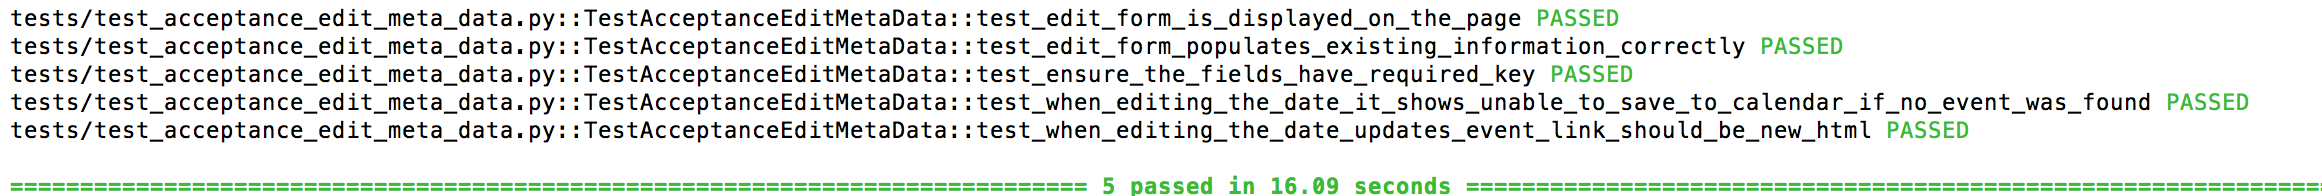
\includegraphics{images/acceptance_test_1}
  \caption{An example of the acceptance tests running. It shows that the time to run the tests have increased considerably.}
  \label{fig:acceptance_test_1}
\end{figure}

In Figure \ref{fig:acceptance_test_1} it shows that the time to run to run 5 tests increased to 16.09 seconds. These tests are costly on time to run, but they ensure that the logic in the view files displays the correct dynamic content.

\section{User Testing}
Due to the application aiming to solve a problem, a set of likely user's were asked to perform a user study of the application. Their responses were analysed and their optinions on whether the software met their aims was collated.

Prior to the actual scheduled user-testing, feedback was given regarding the displaying of the Tesseract output confidence. These ``over the shoulder'' comments were along the lines of: ``It would be great if you could click the identified text and it would automatically populate the text boxes''. This was then implemented as a result from pre-user testing.

Further issues which were identified during the user testing were:
\begin{itemize}
  \item Uploading a JPG image off a phone, which does not have the correct datetime exif key causes the application to fail.
  \item Uploading an image with a previously uploaded filename caused the application to display the old file.
\end{itemize}

These issues were caught and modified thanks to extensive user-testing of the application.

One interesting reflection of the user-case study was that people would not use the application. They were quick to defend the applications quality, but the use-case for them taking notes was not present. They much preferred to write up their notes from the lecture for memory retention.

\section{Tesseract Testing}
Due to there being no code written for the Tesseract training process there were no formal tests conducted for this section. However, what could be tested was how well the Tesseract learned as it progressed through the training processes.

\begin{figure}[h]
  \centering
  \includegraphics{images/tesseract_testing}
  \caption{A simple framework showing the steps of analysing each of the training examples for a statistical measure for how successful the training process was.}
  \label{fig:tesseract_framework}
\end{figure}

Figure \ref{fig:tesseract_framework} shows a simple framework for analysing how well Tesseract trained the data. After the statistics has been collated then a graph was constructed to show the trends.
\begin{figure}[h]
  \centering
\begin{tikzpicture}
\begin{axis}[
    title={Tesseract Training examples compared to their success rate of characters identified vs correct characters},
    xlabel={Training example},
    ylabel={Success rate (\%) },
    xmin=0, xmax=100,
    ymin=0, xmax = 100,
    ytick={0,20,40,60,80,100},
    xtick={0, 9,18,27,36,45,54,63, 72, 81 , 90 , 99},
    xticklabels={1, 2, 3, 4, 5, 6, 7, 8, 9 , 10 , 11 ,12 },
    legend pos=north west,
    ymajorgrids=true,
    grid style=dashed,
]

\addplot[
    color=black,
    mark=square,
    ]
    coordinates {
    (0, 61.4035087719298)(9, 72.2222222222222)(18, 81.1594202898551) (27, 79.1044776119403)(36, 69.7916666666667)(45, 74.6376811594203) (54, 78.5276073619632)(63, 69.75)(72, 78.7878787878788)(81, 66.3341645885287)(90, 65.5737704918033)(99, 75.414364640884)
    };

\addplot [thick, red] table[y={create col/linear regression}]{
    0 61.4035087719298
    9 72.2222222222222
    18 81.1594202898551
    27 79.1044776119403
    36 69.7916666666667
    45 74.6376811594203
    54 78.5276073619632
    63 69.75
    72 78.7878787878788
    81 66.3341645885287
    90 65.5737704918033
    99 75.414364640884
    };
\end{axis}
\end{tikzpicture}
\caption{A graph showing the success rate of the Tesseract training results over 12 examples.}
\label{fig:tesseract_graph}
\end{figure}

Figure \ref{fig:tesseract_graph} shows the output analysed from the Tesseract training. It shows each training example with an associated correct character recognition. The conclusions clearly show that there is no improvement from the Tesseract output after around the 3rd example. A horizontal linear regression line shows that it has peaked at around 72\% correct recognition rate.

\section{Image thresholding Testing}
Due to the nature of the image processing scripts it was quickly realised a methodical approach to testing would not be beneficial, due to almost constant spike work.

TDD would not be performed before considering the design for the image bininarsation script. Instead the testing would consist of a more viaual check of the outputted image to see if the result was clear enough, with little noise. Once the script had been developed to a reasonable level of satisfaction the spike work would cease, and testing would ensue.

The code was re-written and performed using TDD. It involved analysing numpy arrays returned from OpenCV and checking, for instance, if any of the array contained black values.
